\chapter{Exploration of atomistic predictions}
\label{chapter2}

The ANAKIN-ME methodology provides a framework for atom-wise decomposition of molecular energies by using the atomic environment vector (AEV) representation to encode localized chemical interactions.
A decomposition approach allows for efficient, scalable predictions of energy for systems larger than the training data represents.
This is advantageous for simulating large systems, due to the size limitations of \textit{ab initio} computations.
However, this raises a vital question to the efficacy of ML models: how do we assess the reliability of ANI models for systems that exceed the size limitations of QM computations?
Accuracy is well-defined in quantum chemical methods via systematic convergence, 

\section{ANAKIN-ME predictions}
\label{sec:ANI_predictions}

Here I should be writing about the ANI predictions in greater detail than the background information

Add content from pages 5-15 of qualifying exam document -- will need significant rewriting, but the details of the work completed there is useful for filling this section in. 


\subsection{Total energy as a sum of atomic energies}
\label{subsec:total_E_sum_AEs}

Eqn. \ref{eq:total_E_sum_AEs}, where $E_{\text{Total}}$ is the molecular energy prediction, $\varepsilon_i$ is the atomic energy contribution for atom $i$, and $\text{GSAE}_i$ is the ground state atomic energy for atom $i$.
The ground state atomic energies for each atom in the ANI networks are given in \ref{appendix:GSAEs}.

\begin{equation}
    E_{\text{Total}} = \sum_{i}^{\text{atoms}} \varepsilon_i + \text{GSAE}_i
    \label{eq:total_E_sum_AEs}
\end{equation}

\authorRemark{Here you should compare 2x atomic energy predictions to the 2xr predicitons, discuss how the distributions are shifted due to retraining with GSAEs but also note that the distributions are shaped differently, and models do not agree on what atomic energy partition should be.}

\begin{figure}[!ht]
    \centering
    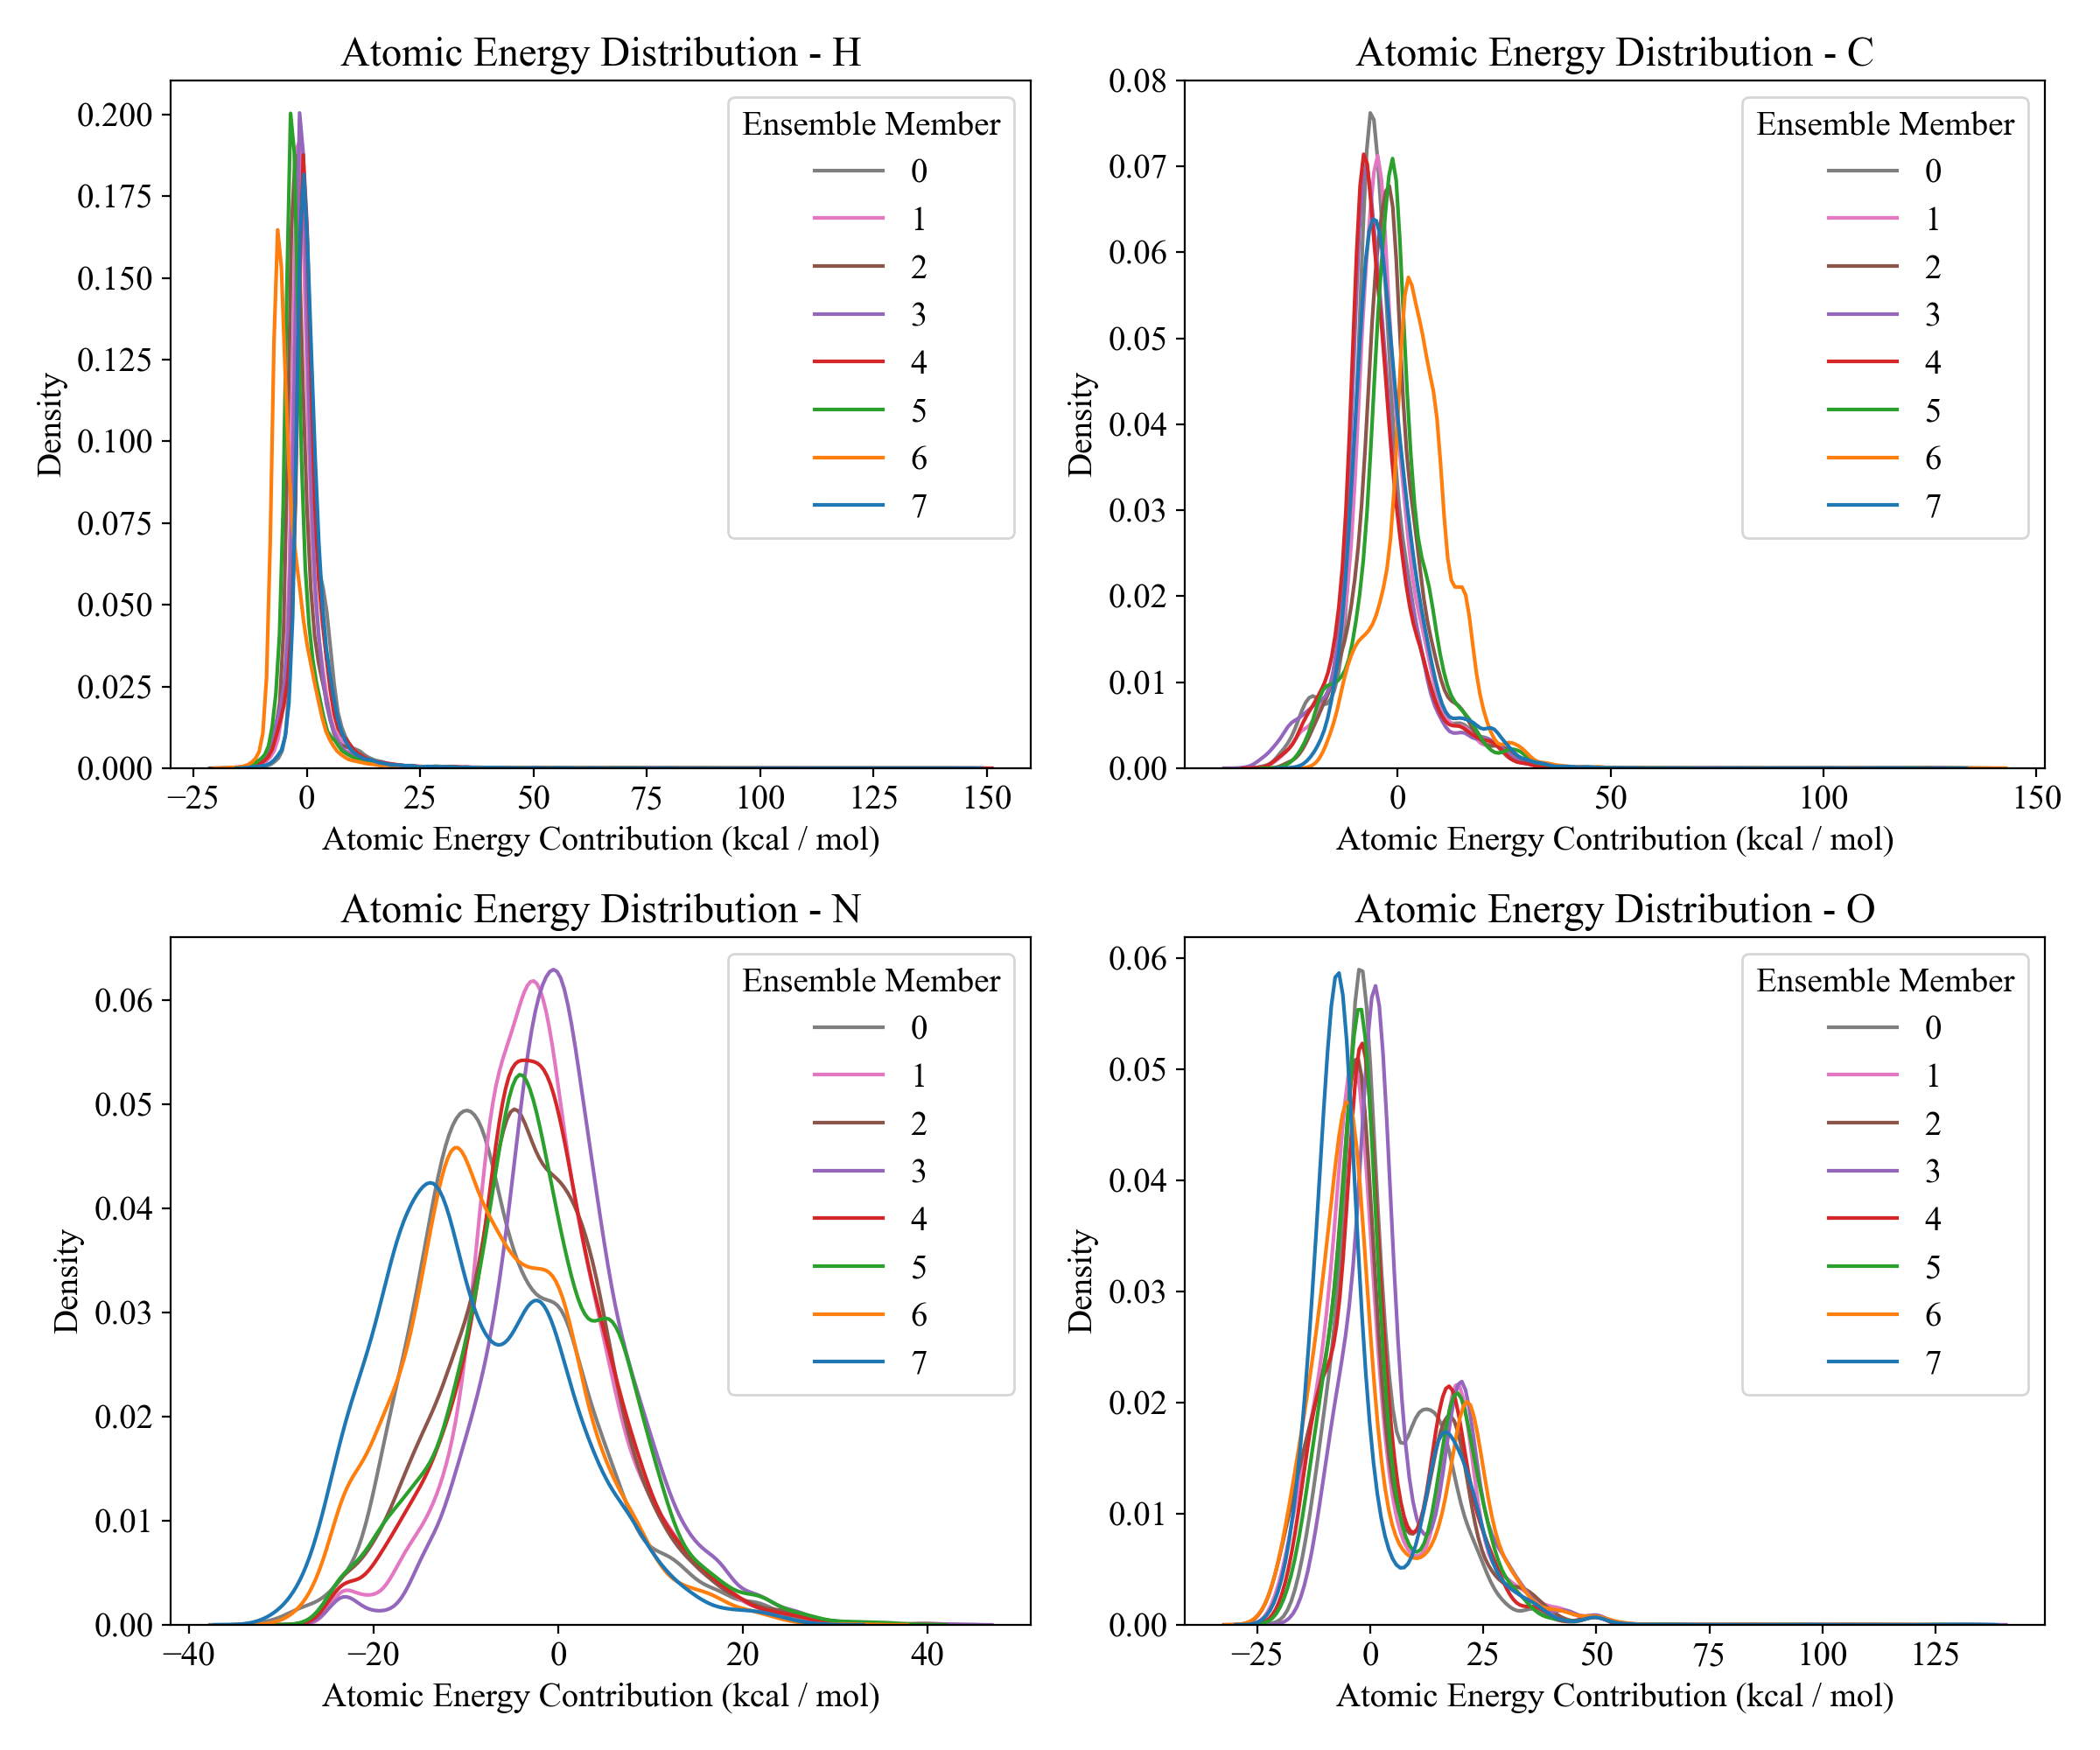
\includegraphics[width=1\linewidth]{Images/2x_outputs/2x_1x-first_ae-per-model.png}
    \caption{Caption}
    \label{fig:2x_ae_per_model}
\end{figure}

\authorRemark{You'll need to write something in between these to have the text spaced out properly.}

\begin{figure}[!ht]
    \centering
    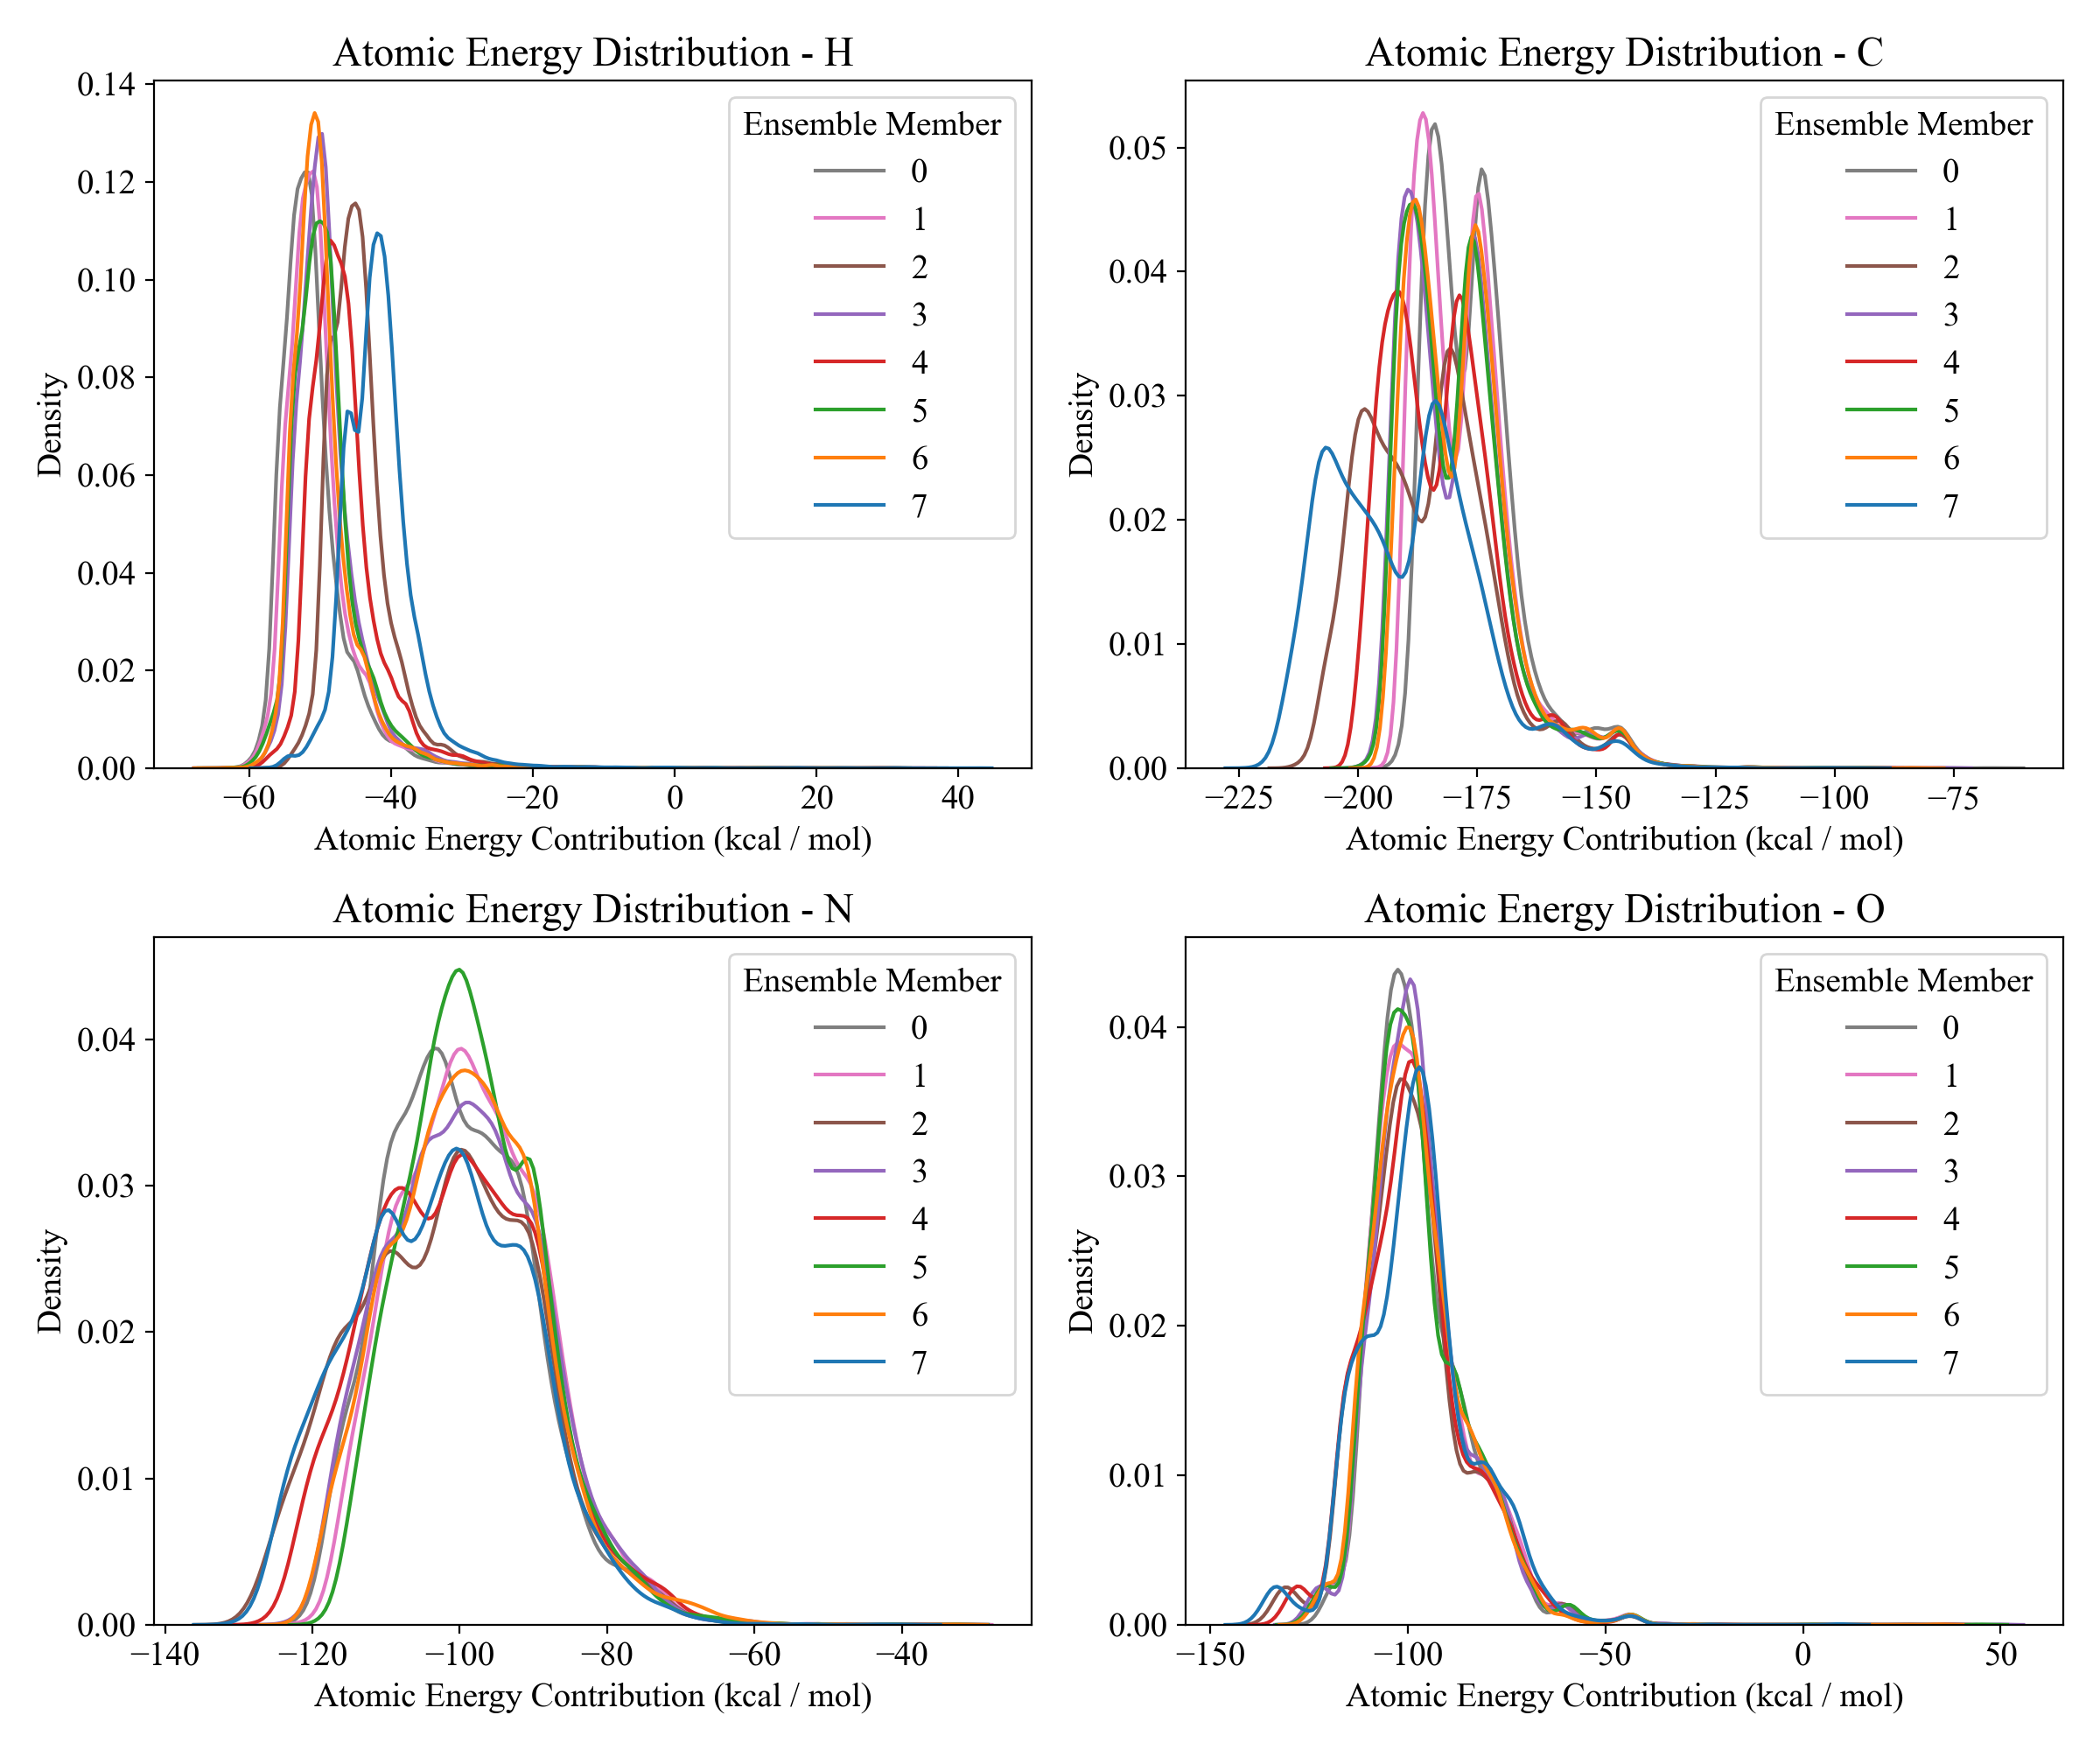
\includegraphics[width=1\linewidth]{Images/2xr_outputs/2xr_1x-first_ae-per-model.png}
    \caption{Caption}
    \label{fig:2xr_ae_per_model}
\end{figure}

Due to the parameters used in training (no biases, GSAEs rather than fitting to SAEs), 2xr is going to be the model used to discuss atomic trends after this.

\subsection{Uncertainty in ANI neural network potentials}
\label{subsec:ANI_uncertainty}

ANI potentials use an ensemble of 8 models.
Predictive uncertainty has been measured in published models using $\hat{rho}$; the value 0.23 kcal/mol was empirically chosen for sampling structures with high-error energy predictions via query by committee (QBC) in the active learning process \cite{ani-1x}.
The QBC, given in Eqn. \ref{eq:energy_qbc}, can be thought of as a binary classifier: 

\begin{equation}
\rho = \frac{\sigma_{E_{\text{Total}}}}{\sqrt{N_{\text{atoms}}}}
\label{eq:energy_qbc}
\end{equation}

\begin{figure}[!hb]
    \centering
    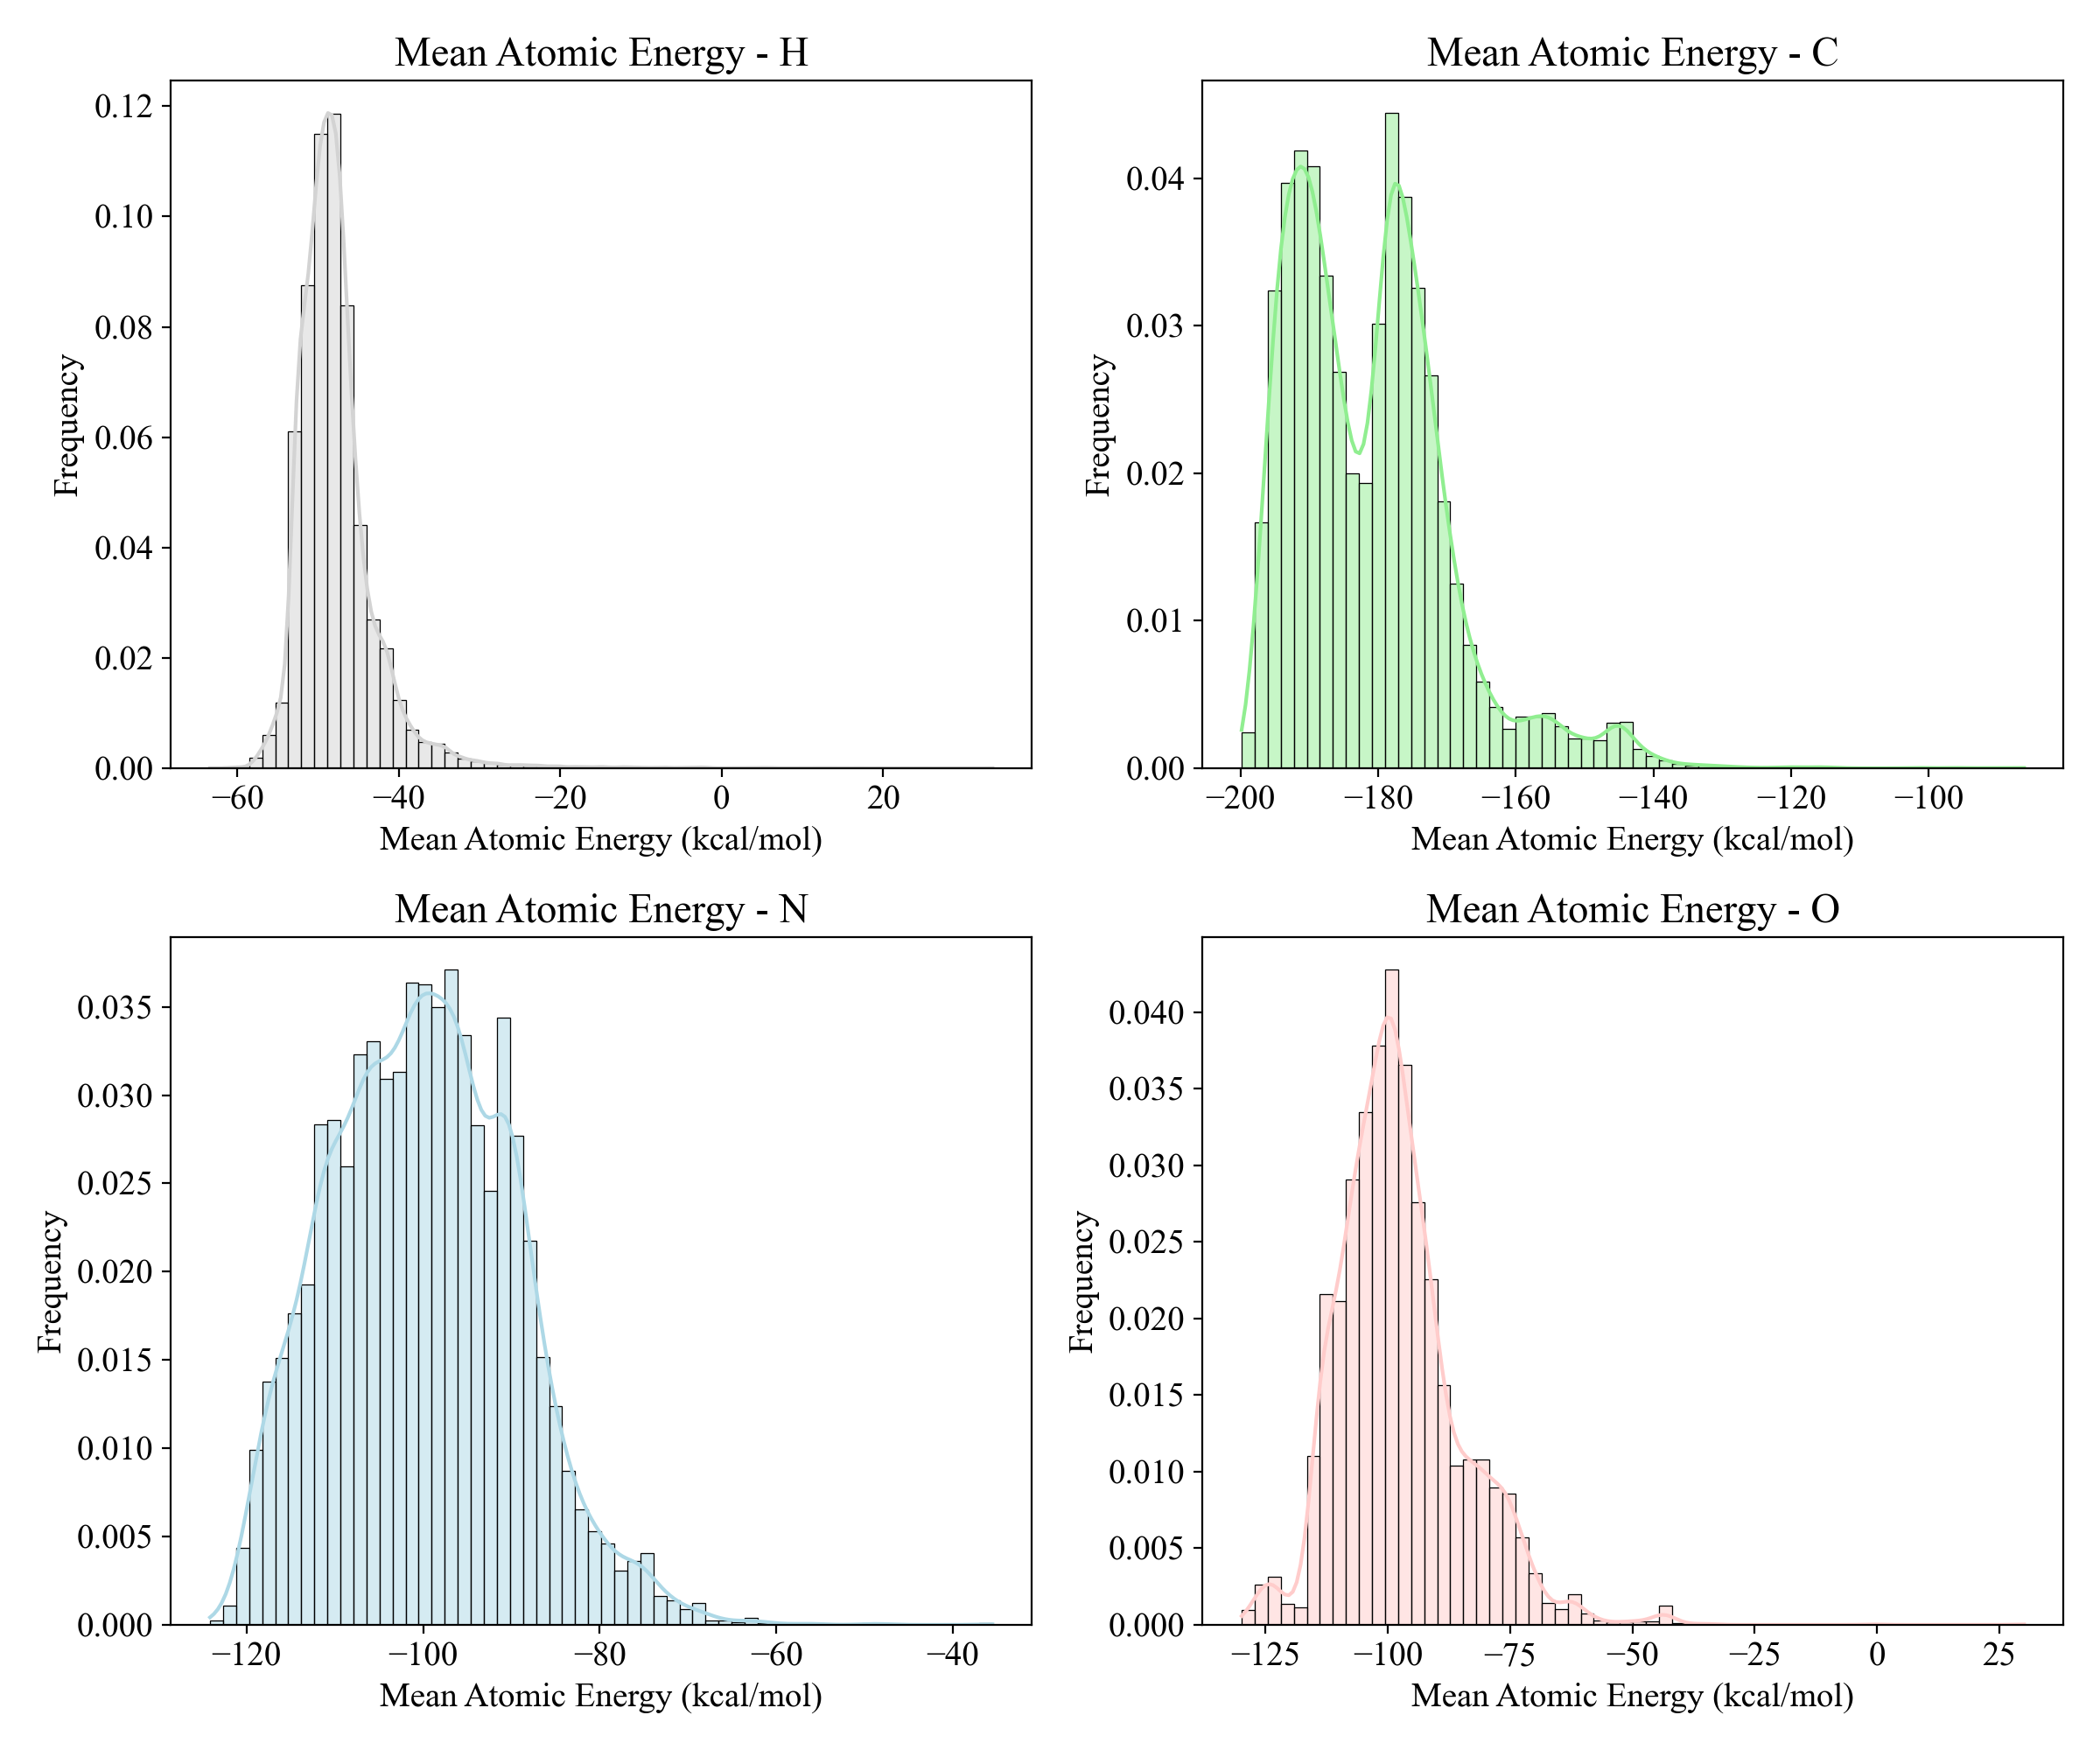
\includegraphics[width=1\linewidth]{Images/2xr_outputs/2xr_1x-first_mean-ae-per-atomtype.png}
    \caption{Caption}
    \label{fig:2xr_1x-first_mean-ae-per-atomtype}
\end{figure}

\subsection{Exploration of the flaws in predicting total energy as a sum of atomic energies}
\label{subsec:flaws_in_atomic_energies}

\authorRemark{MAKE PLOTS OF JUST CARBON STDEV, PLOT LINE ON TOTAL ENERGY STDEV GRAPH}

\begin{equation}
    \label{eq:covariance}
    \text{cov}(x, y) = \mathbb{E}[(x - \mathbb{E}[x])(y - \mathbb{E}[y])]
\end{equation}


\begin{figure}[ht]
    \label{fig:ch4}
    \centering
    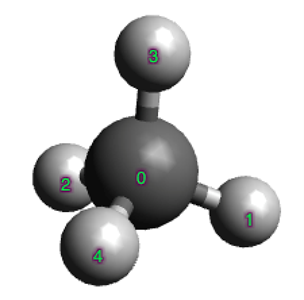
\includegraphics[width=2in]{Images/CH4.png}
    \caption{}
\end{figure}{}

% Tables suck, but this helped me align columns and headers separately:
\begin{table}[!hb]
\centering
\caption{
Atomic energy contributions by atom type in a geometry-optimized molecule of CH\textsubscript{4}, with four equivalent hydrogen atoms. 
Additionally, the sum over all atoms, and that sum after passing through the TorchANI EnergyShifter. 
Values obtained from an ensemble of ANI models (ANI-DR); the last column shows the standard deviation of predictions across the ensemble. 
All values are in kcal/mol.
}\label{tbl:ch4_AEs}
    \begin{tabularx}{\textwidth}{%
    >{\raggedleft\arraybackslash}r  % Numeric
    >{\raggedleft\arraybackslash}r  % Numeric
    >{\raggedleft\arraybackslash}r  % Numeric
    >{\raggedleft\arraybackslash}r  % Numeric
    >{\raggedleft\arraybackslash}r  % Numeric
    }  
      \hline
      Model & Carbon & Hydrogen & Sum of atomic energies & Molecular energy \\
      \hline
      1 & -4.467 & -1.834 & -11.803 & -25413.871 \\
      2 & 15.049 & -6.709 & -11.787 & -25413.855 \\
      3 & 1.656 & -3.352 & -11.754 & -25413.822 \\
      4 & -8.199 & -0.882 & -11.728 & -25413.796 \\
      5 & -7.859 & -0.958 & -11.691 & -25413.759 \\
      6 & 6.757 & -4.636 & -11.787 & -25413.856 \\
      7 & -1.683 & -2.492 & -11.652 & -25413.720 \\
      8 & -4.101 & -1.824 & -11.395 & -25413.463 \\
      Standard deviation & 7.437 & 1.871 & 0.125 & 0.125 \\
      \hline
    \end{tabularx}
\end{table}


\section{Drawback of atomic energy predictions}


\begin{figure}
    \centering
    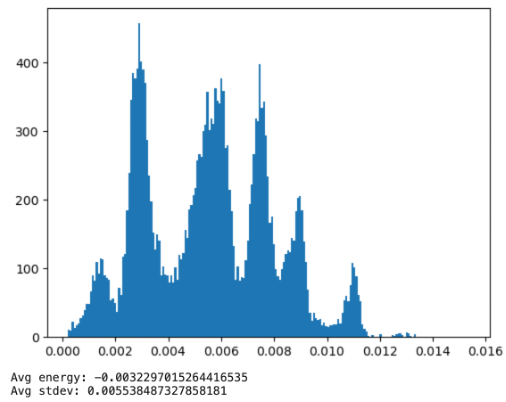
\includegraphics[width=0.5\linewidth]{Images/useful figures/energies/2x_carbon_e_std.png}
    \caption{Caption}
    \label{fig:2x_c_ae_std}
\end{figure}

insert images of hydrogen / carbon / nitrogen / oxygen stdev histograms, 

\section{Need for a practical, physical quantity to estimate uncertainty}

Looking for a correlation between the energy error and the predictive uncertainty of a given \textbf{atomic} quantity.

The ANI models excel at predicting molecular energies, but have also been trained to predict other properties, most notably forces, which are computed as a the second derivative of the potential energy surface. 

\begin{equation}
    Give\ the\ force\ loss\ here
\end{equation}


